% Template for PLoS
% Version 1.0 January 2009
%
% To compile to pdf, run:
% latex plos.template
% bibtex plos.template
% latex plos.template
% latex plos.template
% dvipdf plos.template

\documentclass[10pt]{article}

% amsmath package, useful for mathematical formulas
\usepackage{amsmath}
% amssymb package, useful for mathematical symbols
\usepackage{amssymb}

% graphicx package, useful for including eps and pdf graphics
% include graphics with the command \includegraphics
\usepackage{graphicx}

% cite package, to clean up citations in the main text. Do not remove.
\usepackage{cite}

\usepackage{color} 

% Use doublespacing - comment out for single spacing
%\usepackage{setspace} 
%\doublespacing

% put this in temporarily
\usepackage{algorithm, algorithmicx, algpseudocode} 

% Text layout
\topmargin 0.0cm
\oddsidemargin 0.5cm
\evensidemargin 0.5cm
\textwidth 16cm 
\textheight 21cm

% Bold the 'Figure #' in the caption and separate it with a period
% Captions will be left justified
\usepackage[labelfont=bf,labelsep=period,justification=raggedright]{caption}

% Use the PLoS provided bibtex style
\bibliographystyle{plos2009}

% Remove brackets from numbering in List of References
\makeatletter
\renewcommand{\@biblabel}[1]{\quad#1.}
\makeatother


% Leave date blank
\date{}

\pagestyle{myheadings}
%% ** EDIT HERE **


%% ** EDIT HERE **
%% PLEASE INCLUDE ALL MACROS BELOW

%% END MACROS SECTION

\begin{document}

% Title must be 150 characters or less
\begin{flushleft}
{\Large
\textbf{A Data Driven Framework for Patient-Specific Neural Field Modelling}
}
% Insert Author names, affiliations and corresponding author email.
\\
Dean R. Freestone$^{1,2,3}$, 
Parham Aram$^{4}$, 
Michael Dewar$^{5,\ast}$,
Kenneth Scerri$^{6,\ast}$,
David B. Grayden$^{1,\ast}$,
Visakan Kadirkamanathan$^{4}$
\\
\bf{1} Department of Electrical and Electronic Engineering, University of Melbourne, Melbourne, VIC, Australia
\\
\bf{2} The Bionic Ear Institute, East Melbourne, VIC, Australia
\\
\bf{3} Institute for Adaptive and Neural Computation, University of Edinburgh, Edinburgh, UK
\\
\bf{4} Department of Automatic Control and Systems Engineering, University of Sheffield, Sheffield, UK
\\
\bf{5} Department of Applied Physics and Applied Mathematics, Columbia University, New York, NY, USA
\\
\bf{6} Department of Systems and Control Engineering, University of Malta, Msida, MSD, Malta
\\
$\ast$ E-mail: dfreestone@bionicear.org
\end{flushleft}

% Please keep the abstract between 250 and 300 words
\section*{Abstract}
This paper presents a framework for creating patient-specific neural field models from electrophysiological data. The Wilson and Cowen or Amari style neural field equations are used to form a parametric model, where the parameters are estimated from data. To illustrate the estimation framework, data is generated using the neural field equations incorporating modelled sensors, so a comparison can be made between estimated and true parameters. To facilitate state and parameter estimation, we introduce a method to reduce the continuum neural field model, using a basis function decomposition, to form a finite-dimensional state-space model. Spatial frequency analysis methods are introduced for model selection by systematically specifying the basis function configuration required to capture the dominant characteristics of the neural field. The estimation procedure consists of a two-stage iterative algorithm incorporating the unscented Rauch-Tung-Striebel smoother for state estimation and a least squares algorithm for parameter estimation. The results show that it is possible to reconstruct the neural field and estimate intracortical connectivity and synaptic dynamics with the proposed framework. The results also illustrate the loss of high spatial frequency information as the cost incurred by the model reduction procedure. This framework provides a link between patient-specific neurophysiological data and theoretical neural fields models. This link may lead to greater understanding of cortical dynamics at the meso/macroscopic scale where diseases such as epilepsy are manifested.

% Please keep the Author Summary between 150 and 200 words
% Use first person. PLoS ONE authors please skip this step. 
% Author Summary not valid for PLoS ONE submissions.   
\section*{Author Summary}

\section*{Introduction}
Generating physiologically plausible neural field models are of great importance for studying brain dynamics at the meso/macroscopic scale. While our understanding of the function of neurons is well developed, the overall behaviour of the brain's meso and macro-scale dynamics remains largely theoretical. Understanding the brain at this level is extremely important since it is at this scale that pathologies such as epilepsy, Parkinson's disease and schizophrenia are manifested. 

Mathematical neural field models provide insights into the underlying physics and dynamics of electroencephalography (EEG) and magnetoencephalography (MEG) (see \cite{Deco2008,David2003} for recent reviews). These models have demonstrated possible mechanisms for the genesis of neural rhythms (such as the alpha and gamma rhythms) \cite{Liley1999,RENNIE2000}, epileptic seizure generation \cite{DaSilva2003,Suffczynski2004,Wendling2005} and insights into other pathologies \cite{Moran2008,Schiff2009} that would be difficult to gain from experimental data alone. 

Unfortunately, the use of these models in the clinic has been limited, since they are constructed for ``general'' brain dynamics whereas pathologies almost always have unique underlying patient-specific causes. Patient-specific data from electrophysiological recordings is readily available in the clinical setting, particularly from epilepsy surgery patients, suggesting an opportunity to make the patient-specific link to models of cortical dynamics. Furthermore, recent technological advances have driven an increased level of sophistication in recording techniques, with dramatic increases in spatial and temporal sampling~\cite{Brinkmann2009}. However, the meso/macroscopic neural dynamic state is not directly observable in EEG data, making predictions of the underlying physiology inherently difficult.

For models to be clinically viable, they must be patient-specific. A possible approach to achieve this would be to fit a general continuum neural field model, like the Wilson and Cohen (WC)~\cite{Wilson1973} or Amari~\cite{Amari1977} models or a neural mass model like the Jansen and Ritt model~\cite{Jansen1995}, to patient-specific EEG data. Fitting the neural models to individuals is a highly non-trivial task and, until very recently, has not been reported in the literature. 

An estimation framework for neural field models known as dynamical causal modelling (DCM) \cite{David2003,David2006} has recently been proposed for studying evoked potential dynamics. Via a Bayesian inference scheme, DCM estimates the long range (cortico-cortical) connectivity structure between the specific isolated brain regions that best explains a given data set using the Jansen and Ritt equations. Another recent publication describing a parameter estimation method with a neural field model used an unscented Kalman filter with the WC neural field equations~\cite{schiff2008kalman}. This work takes a system theoretic approach to the neural estimation problem, successfully demonstrating that it is possible to perform state estimation of modified WC equations. This marks the first step in what has the potential to revolutionise the treatment of many neurological diseases where therapeutic electrical stimulation is viable.

We present an extension to the work of Schiff and Sauer~\cite{schiff2008kalman} by establishing a framework for estimating the state of the WC equations for larger scale (more space) systems via a systematic model reduction procedure. In addition, a method is presented for estimating the connectivity structure and the synaptic time dynamics. Until now, model-based estimation of local intracortical connectivity has not been reported in the literature (to the best of the authors' knowledge). Our work builds on recent work which shows that it is possible to estimate local coupling of spatio-temporal systems using techniques from control systems theory and machine learning~\cite{Dewar2009}. The key development of this previous work was to represent the spatiotemporal system as a standard state-space model, with the number of states independent of the number of observations (recording electrodes in this case). In addition, the appropriate model selection tools have been developed~\cite{Scerri2009} allowing for the application of the technique to neural fields. 

Modelling the neural dynamics within this framework has a distinct advantage over the more standard multivariate auto-regressive (MVAR) models: the number of parameters to define the spatial connectivity is considerably smaller than the number of AR coefficients typically required to achieve the required model complexity. 

In this paper, we demonstrate for the first time how intracortical connectivity can be inferred from data, based on a variant of the WC neural field model~\cite{Wilson1973}. This work provides a fundamental link between the theoretical advances in neural field modelling and patient-specific data. The paper proceeds by first deriving the continuum neural field equations in Section~\ref{NeuralModelSection}. Then a finite dimensional neural field model is derived. The model is reduced by approximating the neural field using a set of continuous basis functions, weighted by a finite dimensional state vector. Section~\ref{SpectralAnalysisSection} establishes conditions using spatial frequency analysis for both sensor and basis function spacing and width, such that the dominant dynamics of the neural field can be represented by the reduced model. The state and parameter estimation procedure is described in Section~\ref{StateAndParameterEstimationSection}. The results for the spatial frequency analysis and parameter estimation are then presented in Section~\ref{ResultsSection}. The implications and limitations of this framework are discussed in Section~\ref{DiscussionSection} along with planned future developments.

% You may title this section "Methods" or "Models". 
% "Models" is not a valid title for PLoS ONE authors. However, PLoS ONE
% authors may use "Analysis" 
\section*{Methods}

\subsection{Neural Field Model}\label{NeuralModelSection} 
Neural field models relate mean firing rates of pre-synaptic neural populations to mean post-synaptic membrane potentials. They are popular as they are parsimonious yet have a strong link with the underlying physiology. Each neural population represents a functional cortical processing unit, such as a column. The columnar organisation of the cortex is continuous, where pyramidal cells are members of many columns. In general, cortical structure can be modelled in a physiologically plausible manner as being locally homogeneous (in short range intracortical connectivity) and heterogeneous (in long range cortico-cortical and corticothalamic connectivity)~\cite{Jirsa2009,Qubbaj2007}. In certain regions of the cortex, each column is thought to be connected locally via symmetric short range local excitation with surround inhibition \cite{Braitenberg1998}. For example, this structural organisation is most studied in the visual system, where the surrounding inhibition effectively tunes a cortical column to a particular receptive visual field~\cite{Sullivan2006}. Neural field models are descriptive of a range of neurodynamics of the cortex such as evoked potentials, visual hallucinations and epileptic behaviour~\cite{David2003,Bressloff2001,Breakspear2006}. Field models are also capable of generating complex spatial patterns of activity such as Turing patterns, spirals and travelling oscillations~\cite{Amari1977,Coombes2005,Coombes2007}.

\subsection{Derivation of the Integro-Difference Equation Representation}
The model relates the average number of action potentials $g(\mathbf{r},t)$ arriving at position $\mathbf{r}$ to the local post-synaptic membrane voltage $v(\mathbf{r},t)$. The post-synaptic potentials generated at a neuronal population at location $\mathbf{r}$ by action potentials arriving from all other connected populations at locations $\mathbf{r}'$ can be described by 
\begin{equation}
	\label{SpikesToPotential} v\left( {\mathbf{r},t} \right) = \int_{ - \infty }^t {h\left( {t - t'} \right)g\left( {\mathbf{r},t'} \right)dt'}. 
\end{equation}
The post-synaptic response kernel $h(t)$ is described by 
\begin{equation}
	\label{SynapticRespKernel} h(t) = \eta(t)\exp{\left(-\zeta t\right)}. 
\end{equation}
where $\zeta=\tau^{-1}$, $\tau$ is the synaptic time constant and $\eta(t)$ is the Heaviside step function. Non-local interactions between cortical populations are described by 
\begin{equation}
	\label{RateBasedInteractions} g\left( \mathbf{r},t \right) = \int_\Omega {w\left( \mathbf{r},\mathbf{r}' \right)f\left( v\left( \mathbf{r}',t \right) \right)d\mathbf{r}'}, 
\end{equation}
where $f(\cdot)$ is the firing rate function, $w(\cdot)$ is the spatial connectivity kernel and $\Omega$ is the spatial domain representing a cortical sheet or surface. The connectivity kernel is typically a ``Mexican hat'' function, which describes local excitation and surround inhibition. To demonstrate flexibility in estimation algorithm, a third component of the kernel is introduced describing weak longer-range excitation. An example of the connectivity kernel is shown in in Figure~\ref{fig:2d_kernel}. The exact shape of this kernel is assumed to vary across patients, and hence needs to be inferred from data.
\begin{figure}
   	\begin{center}
   		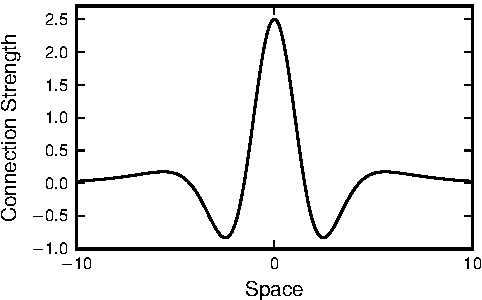
\includegraphics{./Graph/Cross_section_kernel.pdf} 
   	\end{center}
   	\caption{Mexican-hat connectivity kernel, $w(\mathbf{r},\mathbf{r'})$, used in this paper. The function $w(.)$ is rotationally symmetric (isotropic) about zero, hence a cross-section captures the important aspect of the connectivity kernel's shape. The kernel decays asymptotically to zero.}
 	\label{fig:2d_kernel}
   \end{figure}
The firing rate of the presynaptic neurons is related to the postsynaptic membrane potential by the sigmoidal activation function 
\begin{equation}
	\label{ActivationFunction} f\left( v\left( \mathbf{r}', t \right) \right) = \frac{f_{max}}{1 + \exp \left( \varsigma \left( v_0 - v\left(\mathbf{r}',t\right) \right) \right)}. 
\end{equation}
The parameters $f_{max}$ and $v_0$ describe the maximum firing rate and firing threshold of the neural populations respectively. The parameter $\varsigma$ governs the slope of the sigmoid. By substituting equation~\ref{RateBasedInteractions} into \ref{SpikesToPotential} we get the spatiotemporal model 
\begin{equation}
	\label{FullDoubleIntModel} v\left(\mathbf{r},t\right) =
	\int_{-\infty}^t 
	h\left(t - t'\right) \int_\Omega
	w\left(\mathbf{r},\mathbf{r}'\right) 
	f\left( v\left( \mathbf{r}',t \right)\right)
	d\mathbf{r}'dt'.
\end{equation}
To arrive at the final form of the model, we shall express the synaptic response kernel as a Green's function 
\begin{equation}
	\label{GreensFuncDef} Dh\left( t \right) = \delta \left( t \right), 
\end{equation}
where $D=\frac{d}{dt} + \zeta$ is a temporal differential operator and $\delta(t)$ is the Dirac-delta function giving 
\begin{equation}
	\label{FinalFormContinuous} 
	\frac{dv\left( \mathbf{r},t \right)}{dt} + \zeta v\left( \mathbf{r},t \right) = \int_\Omega {w\left( \mathbf{r},\mathbf{r}' \right)f\left( {v\left( \mathbf{r}',t \right)} \right)d\mathbf{r}'}. 
\end{equation}
To arrive at the integro-difference equation (IDE) form of the model, we discretise time using a first-order Euler method (see~\ref{Time Discretization}) giving 
\begin{equation}
	\label{DiscreteTimeModel} 
	v_{t+T_s}\left(\mathbf{r}\right) = 
	\xi v_t\left(\mathbf{r}\right) + 
	T_s \int_\Omega { 
	    w\left(\mathbf{r},\mathbf{r}'\right)
	    f\left(v_t\left(\mathbf{r}'\right)\right) 
	d\mathbf{r}'} 
	+ e_t\left(\mathbf{r}\right), 
\end{equation}
where $T_s$ is the time step, $\xi = 1-\zeta T_s$ and $e_t(\mathbf{r})$ is an $i.i.d.$ disturbance such that $e_t(\mathbf{r})\sim\mathcal{GP}(\mathbf 0,\gamma(\mathbf{r}-\mathbf{r}'))$. Here $\mathcal{GP}(\mathbf 0,\gamma(\mathbf{r}-\mathbf{r}'))$ denotes a spatial Gaussian Process with mean zero and covariance function $\gamma(\mathbf{r}-\mathbf{r}')$~\cite{Rasmussen2005}. This term is added to account for uncertainty and unmodelled inputs. To simplify the notation, the index of the future time sample, $t+T_s$, shall be referred to as $t+1$ throughout the rest of the paper. 

The mapping between the membrane voltage and the electrophysiological data (iEEG/LFP) is modelled using the observation function 
\begin{equation}
    \label{eq:ObservationEquation}
	\mathbf{y}_t =
	\int_{\Omega}{
	    m\left(\mathbf{r}_n-\mathbf{r}'\right)v_t\left(\mathbf{r}'\right)
	d\mathbf{r}'} + 
	\boldsymbol{\varepsilon}_t, 
\end{equation}
where $\mathbf{r}_n$ defines the location of the sensors in the field, $n=1,...,N$ indexes the sensors and $\boldsymbol{\varepsilon}_t \sim \mathcal{N}\left(0,\Sigma_{\varepsilon}\right)$, $\mathcal{N}\left(0,\Sigma_{\varepsilon}\right)$ denotes the multivariate normal distribution with mean zero and covariance matrix $\Sigma_{\varepsilon}$. The output kernel $m(\mathbf{r}-\mathbf{r}')$ governs the sensor pick-up geometry where 
\begin{equation}
	m\left(\mathbf{r}-\mathbf{r}'\right) = \exp{\left(-\frac{(\mathbf{r}-\mathbf{r}')^\top(\mathbf{r}-\mathbf{r}')}{\sigma_m^2}\right)}. 
\end{equation}

\subsection{Derivation of Finite Dimensional State-Space Model}\label{Sect:ReducedModelDerivation}
In order to implement standard estimation techniques, we use a decomposition of the field using a set of Gaussian basis functions that are defined by
\begin{equation}\label{eq:FieldBasisFunction}
	\phi\left(\mathbf{r}-\mathbf{r}'\right) =
\exp{\left(-\frac{(\mathbf{r}-\mathbf{r}')^\top(\mathbf{r}-\mathbf{r}')}{\sigma_{\phi}^2}\right)}. 
\end{equation}
Decomposition allows a continuous field to be represented by a finite-dimensional state vector. This facilitates application of standard nonlinear state estimation methods such as the unscented Kalman filter. The field decomposition is described by 
\begin{equation}
	\label{DefFieldDecomp} v_t\left(\mathbf{r}\right) \approx \boldsymbol{\phi}^{\top}\left(\mathbf{r}\right) \mathbf{x}_t, 
\end{equation}
where $\mathbf{\boldsymbol{\phi}}(\mathbf{r})$ is a vector of Gaussian basis functions that are scaled by the state vector, $\mathbf{x}_t$. An example of the field decomposition is given in Figure~\ref{fig:FieldDecomposition}.%The choice of Gaussian basis functions can be justified by the existence of the so called bump solutions for this class of model, which have a Gaussian shape~\cite{Coombes2005}.
\begin{figure}
   	\begin{center}
   		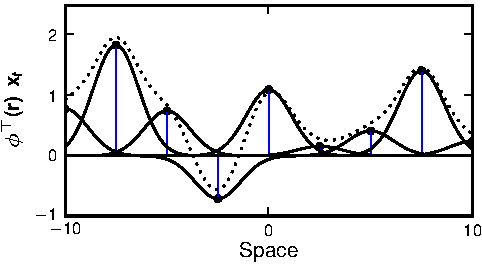
\includegraphics{./Graph/FieldDecomposition.pdf} 
   	\end{center}
   	\caption{An example of a continuous one-dimensional field decomposed by a finite number of basis functions scaled by the state vector.} 
	\label{fig:FieldDecomposition}
   \end{figure}
The width and positioning of the basis functions can be determined by spectral analysis (explained in detail in Section~\ref{SpectralAnalysisSection}). The connectivity kernel can also be decomposed as 
\begin{equation}\label{DefKernelDecomp}
	 w\left(\mathbf{r},\mathbf{r}'\right) =\boldsymbol{\psi}^\top\left(\mathbf{r},\mathbf{r}'\right) \boldsymbol{\theta},
\end{equation}
where $\boldsymbol{\psi}(r,r')$ is a vector of Gaussian basis functions and $\boldsymbol{\theta}$ is a vector of scaling parameters. By assuming a Gaussian isotropic connectivity structure, the kernel basis functions can be written as $\psi(\mathbf{r}-\mathbf{r}')$. We will assume that we know the parametric form of the connectivity basis functions, where the scaling parameters $\boldsymbol{\theta}$ are unknown. Each connectivity basis function can, individually, be considered a layer in the Wilson and Cowan model. Typically, the Mexican hat connectivity kernel is comprised of two basis functions representing local excitation and surround inhibition. To demonstrate the flexibility of the estimation framework, a third basis function is incorporated, corresponding to weaker mid-range excitation. Making substitutions of equations~\ref{DefFieldDecomp} and~\ref{DefKernelDecomp} into~\ref{DiscreteTimeModel} we get 
\begin{equation}
	\label{reduced continuous model}\boldsymbol{\phi}^{\top}(\mathbf{r})\mathbf{x}_{t+1}= T_s\int_\Omega{f(\boldsymbol{\phi}^{\top}(\mathbf{r}')\mathbf{x}_t )\boldsymbol{\psi}^{\top}(\mathbf{r}-\mathbf{r}')d\mathbf{r}'}\boldsymbol{\theta}
	+ \xi\boldsymbol{\phi}^{\top}(\mathbf{r})x_t + e_t(\mathbf{r}). 
\end{equation}
Next we multiply equation~\ref{reduced continuous model} by $\boldsymbol{\phi}(r)$ and integrate over the spatial domain $\Omega$ to get 
\begin{equation}
    \begin{split}
	\label{StartofReduction}
	\lefteqn{ \int_\Omega {\boldsymbol{\phi} \left(\mathbf{r}\right)\boldsymbol{\phi}^{\top}\left(\mathbf{r}\right) d\mathbf{r}} \mathbf{x}_{t+1}=} \\
 &T_s \int_\Omega {\boldsymbol{\phi} (\mathbf{r}) \int_\Omega {\boldsymbol{\psi}^{\top} (\mathbf{r}-\mathbf{r}') f(\boldsymbol{\phi}^{\top}(\mathbf{r}') \mathbf{x}_t ) d\mathbf{r}'}d\mathbf{r}}\boldsymbol{\theta}  \\ & + \xi\int_\Omega {\boldsymbol{\phi}(\mathbf{r})\boldsymbol{\phi}^{\top}(\mathbf{r})d\mathbf{r}} \mathbf{x}_t+
\int_\Omega{\boldsymbol{\phi} (\mathbf{r}) e_t(\mathbf{r})d\mathbf{r}}. 
\end{split}
\end{equation}
Now defining the matrix
\begin{equation}\label{eq:DefGamma}
	\boldsymbol{\Gamma} \triangleq \int_\Omega {\boldsymbol{\phi} \left(\mathbf{r}\right)\boldsymbol{\phi} ^{\top}\left(\mathbf{r}\right)d\mathbf{r}}, 
\end{equation}
and substituting this into equation~\ref{StartofReduction} and cross-multiplying by $\boldsymbol{\Gamma}^{-1}$ gives 
\begin{equation}
    \label{eq:ReducedForm}
    \begin{split}
	 \mathbf{x}_{t+1} = T_s\boldsymbol{\Gamma}^{-1}
	 \int_\Omega \boldsymbol{\phi}(\mathbf{r}) 
	 \int_\Omega \boldsymbol{\psi}^{\top} (\mathbf{r}-\mathbf{r}')f(\boldsymbol{\phi}^{\top}(\mathbf{r}')\mathbf{x}_t) d\mathbf{r}' d\mathbf{r} \boldsymbol{\theta} \\ 
	 + \xi\mathbf{x}_t + \boldsymbol{\Gamma}^{-1} \int_\Omega{\boldsymbol{\phi}(\mathbf{r}) e_t(\mathbf{r})d\mathbf{r}}.
	 \end{split}
\end{equation}
An analytic derivation of the inner product of \emph{n}-dimensional Gaussians is provided in~\ref{ap:InnerProdOfGaussians}. Equation~\ref{eq:ReducedForm} can be simplified by exploiting the symmetry (isotropy) of the connectivity kernel where
\begin{equation}
	\boldsymbol{\psi} (\mathbf{r}-\mathbf{r}') = \boldsymbol{\psi} (\mathbf{r}'-\mathbf{r}).
\end{equation}
To make the simplification, we first define
\begin{equation}\label{eq:DefPsi}
	\boldsymbol{\Psi}(\mathbf{r}') \triangleq T_s\boldsymbol{\Gamma}^{-1}\int_\Omega {\boldsymbol{\phi}(\mathbf{r})\boldsymbol{\psi}^{\top} (\mathbf{r}'-\mathbf{r})d\mathbf{r}},
\end{equation}
which is a constant $L \times n_{\theta}$ matrix that can is defined analytically (see~\ref{ap:ConvOfGaussians} for analytic convolution of two Gaussians), where $L$ is the number of basis functions (and states) and $n_{\theta}$ is the number of connectivity basis functions. Now substituting equation~\ref{eq:DefPsi} into~\ref{eq:ReducedForm} gives
\begin{eqnarray}
	\mathbf{x}_{t+1} = \int_\Omega \boldsymbol{\Psi}(\mathbf{r}') f(\boldsymbol{\phi}^{\top}(\mathbf{r}')\mathbf{x}_t) d\mathbf{r}' \boldsymbol{\theta} + \xi\mathbf{x}_t\nonumber \\
+ \boldsymbol{\Gamma}^{-1} \int_\Omega{\boldsymbol{\phi}(\mathbf{r})e_t(\mathbf{r})d\mathbf{r}}.
\end{eqnarray}
This simplification has transformed the description of the spatial coupling from a convolution, to an inner product. This transformation provides a dramatic increase in simulation speed, which is of great importance considering the computational demands of the estimation algorithm. Now we define the state disturbance as
\begin{equation}\label{eq:Wt} 
	\mathbf{e}_t \triangleq \boldsymbol{\Gamma}^{-1}\int_\Omega {\boldsymbol{\phi} ( \mathbf{r} )e_t( \mathbf{r} )d\mathbf{r}} 
\end{equation}
which is a zero mean normally distributed white noise process with covariance (see~\ref{ColoredNoise})
\begin{equation}
	\boldsymbol\Sigma_e =\mathbf{\Gamma}^{-1}\int_{\Omega}\int_{\Omega}\boldsymbol{\phi}\left(\mathbf r\right) \gamma\left(\mathbf r- \mathbf r' \right)\boldsymbol{\phi}\left(\mathbf r'\right)^{\top}d\mathbf r' d\mathbf r\mathbf{\Gamma}^{- \top}. 
\end{equation}
Under the assumption that the basis function decomposition is accurate, the observation equation of the reduced model is found by substituting equation~\ref{DefFieldDecomp} into~\ref{eq:ObservationEquation} giving
\begin{equation}\label{eq:ReducedObservationEquation}
	\mathbf{y}_t = \int_{\Omega}{m\left(\mathbf{r}_n-\mathbf{r}'\right)\boldsymbol{\phi}^{\top}\left(\mathbf{r}\right) \mathbf{x}_td\mathbf{r}'} + \boldsymbol{\varepsilon}_t. 
\end{equation}
The observation equation is linear and can be written in the more compact form
\begin{equation}\label{ObservationEquation} 
	\mathbf{y}_t = \mathbf{C}\mathbf{x}_t + \boldsymbol{\varepsilon}_t,
\end{equation}
where the observation matrix is 
\begin{equation}
	\mathbf{C} = \left[
	\begin{array}{{ccc}} 
		c_{1,1} & \dots & c_{1,L} \\
		\vdots & \ddots & \vdots \\
		c_{N,1} & \dots & c_{N,L} 
	\end{array}
	\right] 
\end{equation}
and 
\begin{equation}
	c_{i,j} = \int_{\Omega}m(\mathbf{r}_i - \mathbf{r}')\boldsymbol{\phi}_j(\mathbf{r}')d\mathbf{r}'. 
\end{equation}
Now we have the final form of the state-space model where
\begin{equation}\label{eq:finalformstatespacemodel}
	\mathbf{x}_{t+1} = Q(\mathbf{x}_t) +\mathbf{e}_t.
\end{equation}
\begin{equation} 
	\mathbf{y}_t = \mathbf{C}\mathbf{x}_t + \boldsymbol{\varepsilon}_t
\end{equation}
and 
\begin{equation}\label{eq:QmatrixForSigmapoints}
	Q(\mathbf{x}_t) = \int_\Omega \boldsymbol{\Psi}(\mathbf{r}') f(\boldsymbol{\phi}^{\top}(\mathbf{r}')\mathbf{x}_t) d\mathbf{r}' \boldsymbol{\theta} + \xi\mathbf{x}_t.
\end{equation}

\subsection{Spectral Analysis and Model Selection}\label{SpectralAnalysisSection} Spectral analysis has been used to identify both the number of sensors and the number of basis functions required to reconstruct the neural field from sampled observations~\cite{Sanner1992,Scerri2009}. Based on a two-dimensional extension of Shannon's sampling theorem \cite{Peterson1962}, the spatial bandwidth of the observed field can be used to provide a lower bound on both the number of sensors and the number of basis functions required to capture the dominant spectral characteristics of the neural field.

Let the spectral representation of the post-synaptic membrane voltage field at time $t$ be denoted by $V_t(\boldsymbol{\nu})$. According to Shannon's sampling theorem, the field must be spatially band-limited for an accurate reconstruction using spatially discrete observations. Nevertheless, an approximate reconstruction can be obtained if the field is approximately band-limited with 
\begin{equation}
	V_t(\boldsymbol{\nu}) \approx 0 ~ \forall \boldsymbol{\nu} > \boldsymbol{\nu}_c,
\end{equation}
where $\boldsymbol{\nu}_c$ is a cutoff frequency (typically taken as the -3~dB point) with $\boldsymbol{\nu}_c = [\nu_c ~ \nu_c]^\top$. Given such a band-limited field, the distance between adjacent sensors, $\Delta_y$, must satisfy 
\begin{equation}
	\label{eq:MinimumSensorDistance} \Delta_y \leq \frac{1}{2\rho_y\nu_{c}}, 
\end{equation}
where $\rho_y \in \mathbb{R} \ge 1$ is an oversampling parameter. This condition must be satisfied to avoid spatial spectral aliasing effects when reconstructing the hidden dynamic field, $v_t(\mathbf{r})$, using the sampled observations, $\mathbf{y}_t$.

In practice, it is difficult to estimate the bandwidth of the cortex using traditional electrophysiological measurements, possibly preventing us from positioning sensors in accordance to equation~\ref{eq:MinimumSensorDistance}. However, we envisage it may be possible to estimate the spatial bandwidth using other modalities with higher spatial resolution such as, fMRI, NIRS or other optical imaging techniques~\cite{Issa2000}. Nevertheless, spectral aliasing can still be avoided by a proper choice of the spatial sampling distance given the sensors' spectral characteristics. The spatial extent of the sensors results in a spectral low-pass action, thus providing spatial anti-aliasing filtering. Such sensors therefore can only sense the field up to a known spatial bandwidth, denoted by $\boldsymbol{\nu}_{cy}$. Aliasing can then be avoided by positioning the sensors according to equation~\ref{eq:MinimumSensorDistance}, with $\boldsymbol{\nu}_{cy}$ replacing $\boldsymbol{\nu}_c$. 

Although such sensors avoid errors due to aliasing, they attenuate the high spatial frequency variations in the observations. Therefore, any procedure applied to estimate the original field or the underlying connectivity structure from these band-limited observations has the potential to underestimate the high spatial frequency components of both the field and the connectivity kernel. This motivates the use of sensors with wider bandwidths (narrower in space). Nevertheless, this choice would require more sensors in order to satisfy Shannon's sampling theorem for a given spatial region. Therefore, a compromise needs to be found between the bandwidth of the sensor response, the accuracy of the estimation results, the number of sensors used and the computational demands of the estimation procedure when designing experiments.

Similar considerations need to be made regarding the representation of the dynamic field, $v_t(\mathbf{r})$, using the basis function decomposition. Again applying Shannon's sampling theorem, the minimum distance between basis functions must satisfy 
\begin{equation}\label{eq:BasisFunctionSeparation}
	\Delta_{\phi} \leq \frac{1}{2\rho_{\phi}\boldsymbol{\nu}_{cy}}
\end{equation}
where $\rho_{\phi} \in \mathbb{R} \ge 1$ is an oversampling parameter to determine the basis function separation. 

The field basis function widths can also be inferred using spectral considerations~\cite{Sanner1992,Scerri2009}. To demonstrate this, we begin with the two-dimensional Gaussian basis function defined as
\begin{equation}\label{eq:BasisFunctionAtOrigin}
 \phi(\mathbf r)=\mathrm{exp}\left({-\frac{1}{\sigma_{\phi}^2} \mathbf r^\top\mathbf r}\right)
\end{equation}
with the corresponding Fourier transform
\begin{equation}\label{eq:GaussianFT}
\boldsymbol\Phi(\boldsymbol \nu)=\left(\frac{1}{\pi\sigma_{\nu}^2}\right)\mathrm{exp}\left(-\frac{1}{\sigma_{\nu}^2}\boldsymbol\nu^\top \boldsymbol\nu\right),
\end{equation}
where 
\begin{equation}\label{eq:GaussianFTWidth}
	\sigma^2_{\nu} = \frac{1}{\pi^2\sigma_{\phi}^2}. 
\end{equation}
To obtain a 3~dB attenuation at $\boldsymbol\nu_{cy}$, the basis function width, $\sigma^2_{\phi}$, should be chosen to be
\begin{equation}\label{eq:WidthCutOffRelationship}
 \sigma^2_{\phi}= \frac{1}{\pi^2\sigma_{\nu_{cy}}^2},
\end{equation}
where
\begin{equation}\label{eq:WidthFrequencyRelationship}
 \sigma^2_{\nu_{cy}}= \frac{2\boldsymbol\nu_{cy}^\top \boldsymbol\nu_{cy}}{\ln2}.
\end{equation}
This ensures that the basis functions can represent the neural field with frequency content up to $\boldsymbol\nu_{cy}$. Derivations for equations~\ref{eq:GaussianFT} and \ref{eq:WidthFrequencyRelationship} are given in~\ref{ap:FrequencyAnalysis}.

Alternatively, given the basis function width, the spatial cut-off frequency of the field modelled by the decomposition can be determined from spectral analysis. This is particularly useful when considering the spatially distributed basis functions, since Shannon's sampling theorem is derived for perfect point sensors. To calculate the cut-off frequency imposed by the basis functions, $\boldsymbol{\nu}_{c\phi}$, we rearrange equations~\ref{eq:WidthCutOffRelationship} and \ref{eq:WidthFrequencyRelationship} giving
\begin{equation}\label{eq:CutoffFromBasisFuncWidth}
	\boldsymbol{\nu}_{c\phi}=\frac{1}{\pi\sigma_{\phi}}\sqrt{\frac{\ln2}{2}}.
\end{equation} 

Note that for a spatially homogeneous isotropic field, the basis functions can be placed on a regular grid. Thus, the knowledge of the distance between basis functions can be used to determine the total number of basis functions required to represent a known spatial region.

\subsection{State and Parameter Estimation}\label{StateAndParameterEstimationSection} In this section we describe the procedure for estimating the states, $\mathbf{x}_t$, the connectivity kernel parameters, $\boldsymbol \theta$, and the synaptic dynamics, $\xi$. The estimation process is a two part iterative algorithm, consisting of a state estimation step followed by a parameter estimation step. At each iteration, the sequence of estimated state vectors is used to update the parameter set. The resulting parameters are then used when estimating the new state vector sequence for the next iteration. The procedure stops when the parameters converge. The algorithm is initialised using a bounded random state vector sequence guaranteeing that the initial estimated parameter set forms a stable kernel.

The unscented Rauch-Tung-Striebel smoother (URTSS)~\cite{Sarkka2010} is used for the state estimation. The URTSS incorporates an unscented Kalman filter (UKF)~\cite{Julier1997, Merwe2003} in a forward iteration to estimate posterior states, $\hat{\mathbf x}_t^{f}$, followed by a backward iteration to compute the smoothed state estimates, $\hat{\mathbf x}_t^{b}$. The first and the second order moments of the predicted state are captured by propagating the so-called sigma points through the state equation. The sigma points, $\mathcal X_i$, are calculated using the unscented transform as follows:
\begin{equation}\label{eq:sigmapoints1}
	\mathcal X_{0}=\bar x 
\end{equation}
\begin{equation}
	\mathcal X_{i}=\bar x+\left(\sqrt{( L + \lambda)\mathbf P_x}\right)_i, \quad i=1, \dots, L 
\end{equation}
\begin{equation}\label{eq:sigmapoints2}
	\mathcal X_{i}=\bar x-\left(\sqrt{( L + \lambda)\mathbf P_x}\right)_{i- L}, \quad i= L+1, \dots, 2 L 
\end{equation}
where $\bar x$ represents either $\hat{\mathbf x}_t^{f}$ or $\hat{\mathbf x}_t^{b}$, $\mathbf{P}_x$ is the corresponding covariance matrix from the filtering or smoothing, $\left(\sqrt{( L + \lambda)\mathbf P_x}\right)_i$ is the $i^{th}$ column of the weighted matrix square root of $\mathbf P_x$ and $L$ is the dimension of the state space. The total number of sigma points is $2L+1$. The scaling parameter, $\lambda$, is defined as 
\begin{equation}\label{eq:sigmapoints3}
	\lambda=\alpha^2( L+\kappa) - L, 
\end{equation}
where the constant $\alpha$ determines the spread of the sigma points, $\beta$ incorporates prior knowledge of the distribution of $\mathbf{x}$ and $\kappa$ is an additional scaling parameter (see~\cite{Haykin2001} for more details). 

The sigma vectors are propagated through the system equations and weighted to form the predicted mean and covariance. The weights are calculated by 
\begin{equation}
	\mathbf W_0^{(m)}=\frac{\lambda}{ L+\lambda} 
\end{equation}
\begin{equation}
	\mathbf W_0^{(c)}=\frac{\lambda}{ L+\lambda}+(1-\alpha^2+\beta) 
\end{equation}
\begin{equation}
	\mathbf W_i^{(m)}=\mathbf W_i^{(c)}=\frac{1}{2( L+\lambda)} \quad i=1, \dots, 2L, 
\end{equation}
where the superscripts $m$ and $c$ stand for mean and covariance. Since the observation equation is linear (equation~\ref{ObservationEquation}) the standard Kalman Filter update equations are used to correct the predicted states. The state estimates from forward filtering are used to form a new set of sigma points for the smoother, as described above. To compute the smoother gain, the cross-covariance matrix of the states, $\mathbf M$, is also computed. A summary of the URTSS procedure is given in Algorithm~\ref{UKFAlgorithm}. It should be noted that the disturbance, $\mathbf{e}_t$ and the measurement noise, $\boldsymbol{\varepsilon}_t$, are additive. Therefore, the additive form of the URTSS is used, instead of augmenting the state vector with the noise terms with the added benefit of reducing the dimension and the number of sigma points required in the algorithm.
\begin{algorithm}
	\begin{small}
	\caption{The Unscented RTS Smoother}\label{UKFAlgorithm} 
	\begin{algorithmic}[1] 
		\State Forward initialisation 
		\begin{equation*}
		 \hat{\mathbf x}_0, \mathbf P_0 
		\end{equation*}
		\State Forward iteration: for $t \in \left\lbrace 0,\cdots, T\right\rbrace $,
		calculate the sigma points $\mathcal X_{i,t}^f$ using equations \ref{eq:sigmapoints1}-\ref{eq:sigmapoints3} and propagate through equation~\ref{eq:QmatrixForSigmapoints}
% 		\begin{small}
		\begin{equation*}
			\mathcal X_{i,t+1}^{f-}=Q(\mathcal X_{i,t}^f) \quad i=0, \dots, 2L
		\end{equation*}
% 		\end{small}
		calculate the predicted state and the predicted covariance matrix
		\begin{equation*}
			\hat{\mathbf x}_{t+1}^{f-}=\sum_{i=0}^{2L} W_i^{(m)}\mathcal X_{i,t+1}^{f-} 
		\end{equation*}
		\begin{equation*}
			\mathbf P_{t +1}^{f-}=\sum_{i=0}^{2L} W_i^{(c)}(\mathcal X_{i,t+1}^{f-}-\hat{\mathbf x}_{t +1}^{f-})(\mathcal X_{i,t+1}^{f-}-\hat{\mathbf x}_{t +1}^{f-})^\top+\boldsymbol \Sigma_e 
		\end{equation*}
		compute the filter gain, the filtered state and the filtered covariance matrix using the standard Kalman Filter update equations
		\begin{equation*}
			\mathcal K_{t+1}=\mathbf P_{t +1}^{f-}\mathbf C ^\top(\mathbf C \mathbf P_{t +1}^{f-}\mathbf C ^\top+\boldsymbol \Sigma_{\epsilon})^{-1} 
		\end{equation*}
		\begin{equation*}
			\hat{\mathbf x}_{t+1}^{f}=\hat{\mathbf x}_{t+1}^{f-}+\mathcal K_{t+1}(\mathbf y_{t+1}-\mathbf C\hat{\mathbf x}_{t +1}^{f-}) 
		\end{equation*}
		\begin{equation*}
			\mathbf P_{t+1}^f=(\mathbf I - \mathcal K_{t+1}\mathbf C)\mathbf P_{t +1}^{f-} 
		\end{equation*}
		\State Backward initialisation 
		\begin{equation*}
			\mathbf P_T^b= \mathbf P_T^f, \quad \hat{\mathbf x}^b_T= \hat{\mathbf x}^f_T 
		\end{equation*}
		\State Backward iteration: for $t \in \left\lbrace T-1, \cdots, 0 \right\rbrace $ calculate the sigma points $\mathcal X_{i,t}^b$ and propagate them through equation \ref{eq:QmatrixForSigmapoints}
		\begin{equation*}
			\mathcal X_{i,t+1}^{b-}=Q(\mathcal X_{i,t}^b) \quad i=0, \dots, 2L
		\end{equation*}
		 compute the predicted state, the predicted covariance matrix and the cross-covariance matrix
		\begin{equation*}
			\hat{\mathbf x}_{t+1}^{b-}=\sum_{i=0}^{2L} W_i^{(m)}\mathcal X_{i,t+1}^{b-} 
		\end{equation*}
		\begin{equation*}
			\mathbf P_{t +1}^{b-}=\sum_{i=0}^{2L} W_i^{(c)}(\mathcal X_{i,t+1}^{b-}-\hat{\mathbf x}_{t +1}^{b-})(\mathcal X_{i,t+1}^{b-}-\hat{\mathbf x}_{t +1}^{b-})^\top+\boldsymbol \Sigma_e 
		\end{equation*}
		\begin{equation*}
			\mathbf M_{t +1}=\sum_{i=0}^{2L} W_i^{(c)}(\mathcal X_{i,t}^{b-}-\hat{\mathbf x}_{t}^{f})(\mathcal X_{i,t+1}^{b-}-\hat{\mathbf x}_{t+1}^{b-})^\top 
		\end{equation*}
		 Compute the smoother gain, the smoothed state and the smoothed covariance matrix
		\begin{equation*}
			\mathbf S_t=\mathbf M_{t +1}\left[ \mathbf P_{t +1}^{b-}\right] ^{-1} 
		\end{equation*}
		\begin{equation*}
			\hat{\mathbf x}_t^b=\hat{\mathbf x}_t^f+\mathbf S_t\left[\hat{\mathbf x}_{t+1}^{b}-\hat{\mathbf x}_{t+1}^{b-}\right] 
		\end{equation*}
		\begin{equation*}
			\mathbf P_{t}^{b}=\mathbf P_{t}^{f}+\mathbf S_t\left[\mathbf P_{t+1}^{b}-\mathbf P_{t+1}^{b-} \right]\mathbf S_t^\top 
		\end{equation*}
	\end{algorithmic}
\end{small}
\end{algorithm}

Although the system is nonlinear, the parameters of the system are linear with respect to the state. This feature is exploited by our procedure where the parameter estimation uses a least squares (LS) method that minimises the sum of the squared errors (of a predicted state update) with each new estimate of the state vector sequence. To create the least squares parameter estimator, we first define the $L \times n_{\theta}$ matrix
\begin{equation}
	\mathbf{q}(\mathbf{x}_t) = \int_\Omega \boldsymbol{\Psi}(\mathbf{r}') f(\boldsymbol{\phi}^{\top}(\mathbf{r}')\mathbf{x}_t) d\mathbf{r}'.
\end{equation}
Now given a state estimate sequence from an iteration of the URTSS, we can write
\begin{eqnarray*}
	\mathbf x_{1} &=& \mathbf{q}(\mathbf x_0) \boldsymbol{\theta}+\xi\mathbf x_0+\mathbf e_0 \\
	\mathbf x_{2} &=& \mathbf{q}(\mathbf x_1) \boldsymbol{\theta}+\xi\mathbf x_1+\mathbf e_1  \\
	&\vdots& \\
	\mathbf x_{T}&=&\mathbf{q}(\mathbf x_{T-1}) \boldsymbol{\theta}+\xi\mathbf x_{T-1}+\mathbf e_{T-1}. 
\end{eqnarray*}
This can be written in the compact form
\begin{equation}
	\mathbf Z=\mathbf X \mathcal W+\mathbf{e}, 
\end{equation}
where
\begin{small}
\begin{equation*}
	\mathbf Z=\left[
	\begin{array}{cccc}
		\mathbf x_{1}\\
		\mathbf x_{2}\\
		\vdots\\
		\mathbf x_{T}
	\end{array}
	\right],\quad \mathbf X=\left[
	\begin{array}{cccc}
		\mathbf q(\mathbf x_0)& \mathbf x_{0}\\
		\mathbf q(\mathbf x_1)& \mathbf x_{1}\\
		\vdots & \vdots\\
		\mathbf q(\mathbf x_{T-1})& \mathbf x_{T-1}
	\end{array}
	\right] 
\end{equation*}
\end{small}
and
\begin{small}
\begin{equation*}
\quad \mathcal W=\left[
	\begin{array}{cc}
		\boldsymbol{\theta} \\
		\xi
	\end{array}
	\right],\quad \mathbf{e}=\left[
	\begin{array}{cccc}
		\mathbf e_0\\
		\mathbf e_1\\
		\vdots\\
		\mathbf e_{T-1}
	\end{array}
	\right].
\end{equation*}
\end{small}
Following this, the LS parameter estimates, $ \mathcal{\hat{W}}$, are
\begin{equation}
	\mathcal{\hat{W}}=(\mathbf X^\top\mathbf X)^{-1}\mathbf X^\top\mathbf Z. 
\end{equation}

% Results and Discussion can be combined.
\section*{Results}

\subsection*{Subsection 1}

\subsection*{Subsection 2}

\section*{Discussion}



% Do NOT remove this, even if you are not including acknowledgments
\section*{Acknowledgments}


% \section*{References}
% The bibtex filename
\bibliography{BrainIDE}

\section*{Figure Legends}
%\begin{figure}[!ht]
%\begin{center}
%%\includegraphics[width=4in]{figure_name.2.eps}
%\end{center}
%\caption{
%{\bf Bold the first sentence.}  Rest of figure 2  caption.  Caption 
%should be left justified, as specified by the options to the caption 
%package.
%}
%\label{Figure_label}
%\end{figure}


\section*{Tables}
%\begin{table}[!ht]
%\caption{
%\bf{Table title}}
%\begin{tabular}{|c|c|c|}
%table information
%\end{tabular}
%\begin{flushleft}Table caption
%\end{flushleft}
%\label{tab:label}
% \end{table}

\end{document}

